
\documentclass[preprint,12pt,a4]{standalone}
\usepackage{geometry}   % my added package "geometry"
\geometry{letterpaper,tmargin=1in,bmargin=1in,lmargin=2.5cm,rmargin=2.5cm}
\usepackage{tikz}
\usetikzlibrary{calc,patterns,arrows.meta,shapes.arrows,intersections,positioning}
\usetikzlibrary{decorations.pathmorphing,backgrounds,fit,petri}
\usepackage{standalone}
\begin{document}
	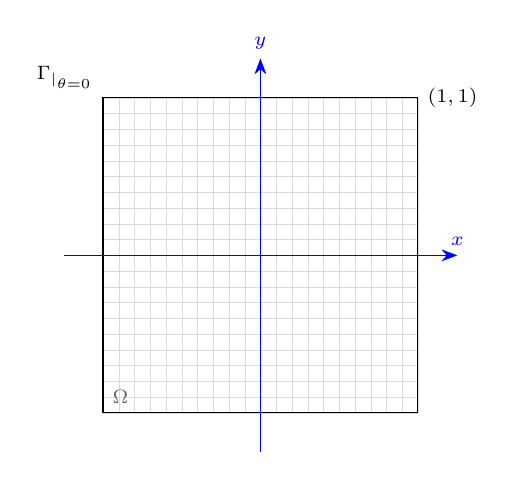
\begin{tikzpicture} [{place/.style={rectangle,draw=blue!50,fill=blue!20,ultra thin,inner sep=0.8mm}},{place2/.style={circle,draw=black!50,ultra thin,inner sep=0.8mm}},{linest/.style={color=gray,ultra thin}}]
	%%coordinates of corners of Beam
	\coordinate (A) at (-2.0,-2.0);
	\coordinate (B) at (2.0,-2.0);
	\coordinate (D) at (2.0,2.0);
	\coordinate (E) at (-2.0,2.0);
	

	%%mesh
	\draw [line width=0.1pt,gray!30,step=2mm](A) grid (D);
	%%Beam	
	\draw [color=black](A)node [above right,color = black!60,font=\scriptsize] {$\boldsymbol{\Omega}$} -- (B)--(D)node [right,color = black,font=\scriptsize] {$(1,1)$} --(E)node [above left,color = black,font=\scriptsize] {$\boldsymbol{\Gamma}_{|_{\theta=0}}$} --(A);
	
	%%axes
	\draw [-{Stealth[length=2mm]},help lines,blue] ($(A)-(0.5,-2)$) -> ($(B)+(0.5,2)$) node [above,color = blue,font=\scriptsize] {$x$};
		\draw [-{Stealth[length=2mm]}, help lines,blue] ($(A)+(2.0,-0.5)$) -> ($(D)+(-2,0.5)$) node [above,color = blue,font=\scriptsize] {$y$};

	\end{tikzpicture}
\end{document}